% The generic preamble
\documentclass[10pt,letterpaper,fleqn,titlepage]{report}

% Define packages to use
\usepackage{natbib}
\usepackage[dvips]{graphicx,color}
\usepackage{amsmath,amssymb}
\usepackage{bm}
\usepackage{caption}
\usepackage{xr}
\usepackage{ifthen}
\usepackage[dvipdfm,colorlinks,linkcolor=blue,citecolor=blue,urlcolor=blue]{hyperref}
\usepackage{fancybox}
\usepackage{textcomp}
\usepackage{fancyhdr}
\usepackage{titlesec}
\usepackage{multirow}
\usepackage{alltt}
\usepackage{svn}
\usepackage{longtable}

\titleformat{\chapter}[frame]
  {\normalfont}
  {\filright\slshape\Huge\enspace\thechapter\enspace}
  {8pt}
  {\normalfont\Huge\filcenter\slshape\sffamily} 

\titleformat{\section}[hang]
  {\normalfont}
  {\filright\sffamily\bfseries\Large\thesection}
  {5pt}
  {\normalfont\Large\filright\sffamily\bfseries}[\vspace{2pt}\titlerule]

\titleformat{\subsection}[hang]
  {\normalfont}
  {\filright\slshape\sffamily\large\thesubsection}
  {5pt}
  {\normalfont\large\filright\slshape\sffamily} 
  
% Redefine default page
\setlength{\textheight}{9.0in}  % 1" above and below
\setlength{\textwidth}{6.75in}   % 0.5" left and right
\setlength{\oddsidemargin}{-0.25in}
\setlength{\topmargin}{0.0pt}
\setlength{\headsep}{16.0pt}

% Redefine default paragraph
\setlength{\parindent}{0pt}
\setlength{\parskip}{1.5ex plus 0.5ex minus 0.2ex}

% Define caption width and default fonts
\setlength{\captionmargin}{0.5in}
\renewcommand{\captionfont}{\sffamily}
\renewcommand{\captionlabelfont}{\bfseries\sffamily}

% Defined commands
\newcommand{\superscript}[1]{\ensuremath{^\textrm{#1}}}
\newcommand{\subscript}[1]{\ensuremath{_\textrm{#1}}}
\newcommand{\invcm}{\textrm{cm\superscript{-1}}}
\newcommand{\micron}{\ensuremath{\mu\textrm{m}}}
\newcommand{\textbfm}[1]{\boldmath\ensuremath{#1}\unboldmath}
\newcommand{\water}{\textrm{H\subscript{2}O}}
\newcommand{\carbondioxide}{\textrm{CO\subscript{2}}}
\newcommand{\ozone}{\textrm{O\subscript{3}}}
\newcommand{\methane}{\textrm{CH\subscript{4}}}
\newcommand{\nitrousoxide}{\textrm{N\subscript{2}O}}
\newcommand{\carbonmonoxide}{\textrm{CO}}

% Define how equations are numbered
\numberwithin{equation}{chapter}
\numberwithin{figure}{chapter}
\numberwithin{table}{chapter}

% Space/nudging commands
\newcommand{\rb}[1]{\raisebox{1.5ex}[0pt]{#1}}

%Redefine the enumerate environment to decrease the item spacing.
\let\oldenumerate=\enumerate
\let\endoldenumerate=\endenumerate
\renewenvironment{enumerate}{%
  \begin{oldenumerate}%
    \setlength{\itemsep}{0ex}%
  }%
  {%
  \end{oldenumerate}%
  }

% Define a command for title page author email footnote
\newcommand{\email}[1]
{%
  \renewcommand{\thefootnote}{\alph{footnote}}%
  \footnote{#1}
  \renewcommand{\thefootnote}{\arabic{footnote}}
}

% Redefine the maketitle macro
\makeatletter
\renewcommand{\maketitle}
{%
  \thispagestyle{empty}
  \vspace*{1in}
  \begin{center}%
     \sffamily
     {\huge\bfseries Joint Center for Satellite Data Assimilation\par}%
  \end{center}
  \begin{flushleft}%
     \sffamily
     \vspace*{0.5in}
     {\Large\bfseries CRTM: \@title\par}%
     \medskip
     {\large\@author\par}%
     \medskip
     {\large\@date\par}%
     \bigskip\hrule\vspace*{2pc}%
  \end{flushleft}%
  \newpage
  \setcounter{footnote}{0}
}
\makeatother


% Define a command for a DRAFT watermark
\usepackage{eso-pic}
\newcommand{\draftwatermark}
{
  \AddToShipoutPicture{%
    \definecolor{lightgray}{gray}{.85}
    \setlength{\unitlength}{1in}
    \put(2.5,3.5){%
      \rotatebox{45}{%
        \resizebox{4in}{1in}{%
          \textsf{\textcolor{lightgray}{DRAFT}}
        }
      }
    }
  }
}


% Generic fixed font command
\newcommand{\f}[1]{\texttt{#1}}

% Title info
\title{Subversion Repository Guide}
\author{Paul van Delst\email{paul.vandelst@noaa.gov}\\JCSDA/EMC/SAIC}
\date{September, 2008}


%-------------------------------------------------------------------------------
%                            Ze document begins...
%-------------------------------------------------------------------------------
\begin{document}
\maketitle

\hyperbaseurl{https://svn.ncep.noaa.gov/emc/}

\draftwatermark

% The tables of content
%======================
\setcounter{page}{1}
\pagenumbering{roman}
  \tableofcontents\newpage
  \listoffigures\newpage
  \listoftables\newpage
\pagenumbering{arabic}
\setcounter{page}{1}


\chapter{Introduction}
%=====================
This document describes the CRTM subversion repository and how to set up your environment to allow you to build the CRTM library, and any associated programs, directly in your working copy. It is assumed the user is familiar with Subversion.

The CRTM is one of many projects in main EMC repository on the subversion server \texttt{svn.ncep.noaa.gov}. The location of the CRTM project repository is \f{https://svn.ncep.noaa.gov/emc/crtm}. Note that, as of September 2008, the EMC repository is still behind the NCEP firewalls and access is available only to users on the NCEP network, or via a VPN connection into the NCEP network.


\chapter{Repository Organisation}
%================================
If you access the repository via your browser, you should see something like figure \ref{fig:main_repository}, where the repository is organised into the usual \f{trunk}, \f{branches}, and \f{tags} subdirectories.
\begin{figure}[htb]
  \centering
  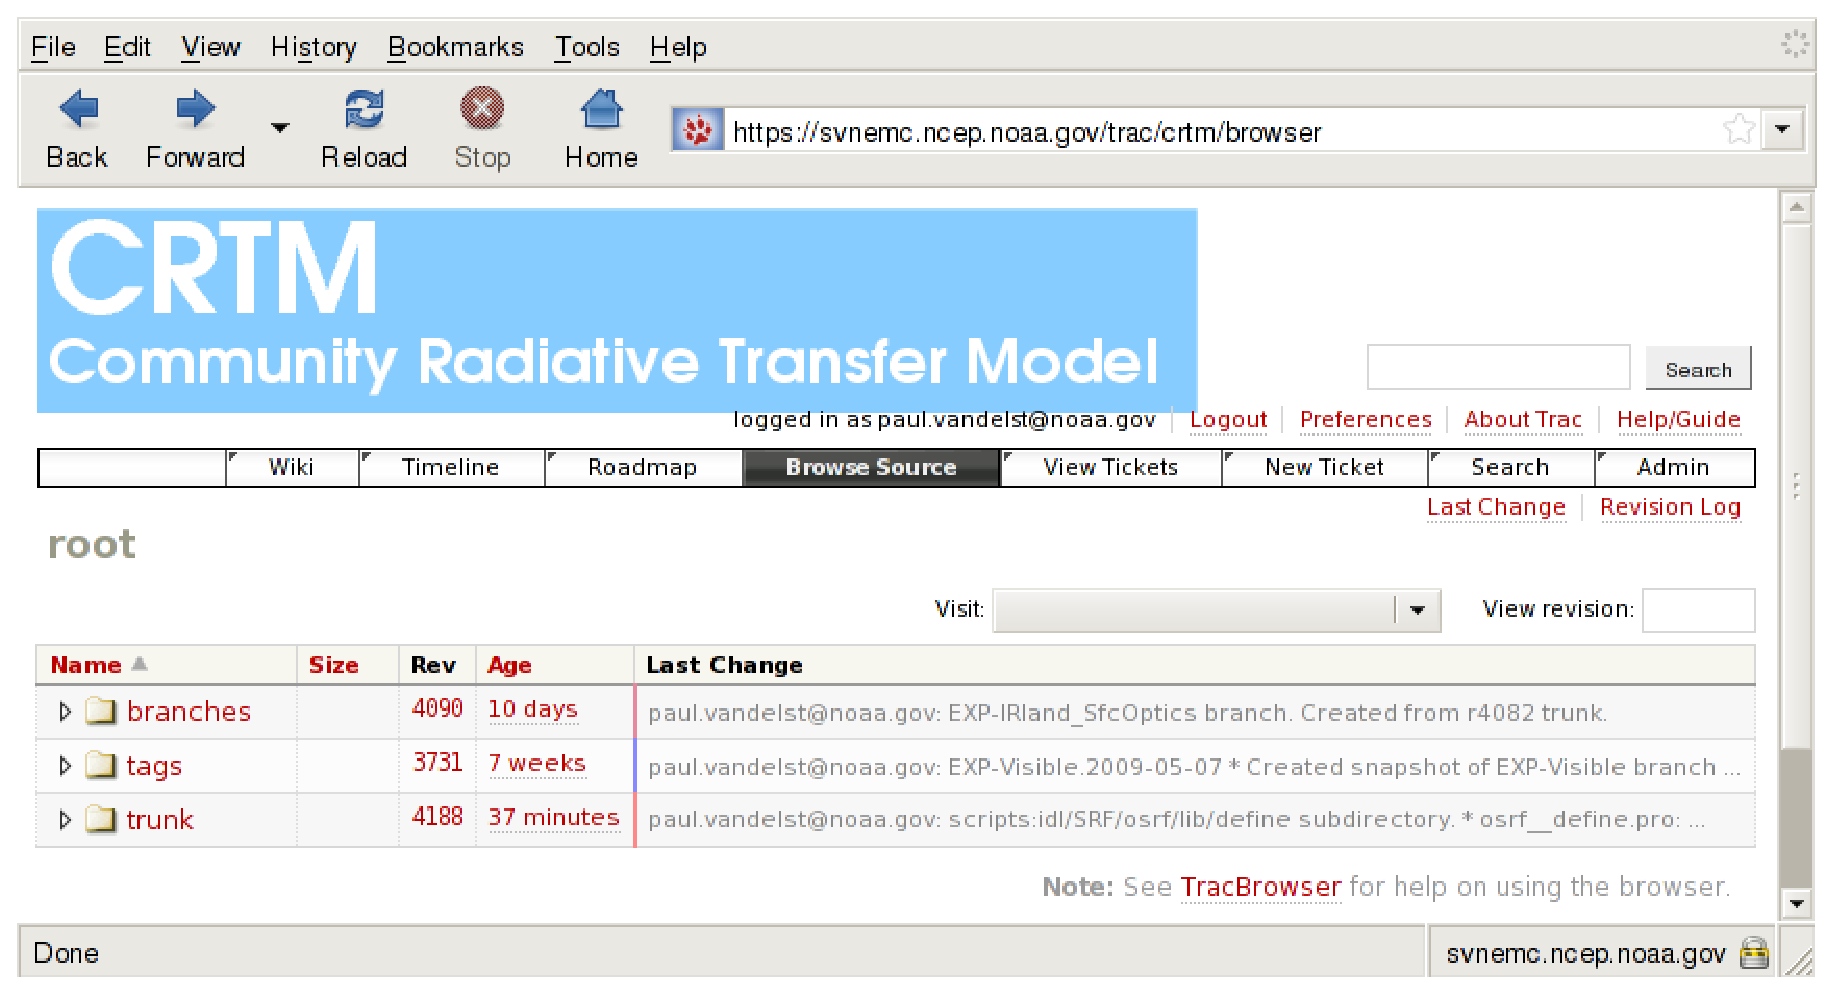
\includegraphics[scale=0.5]{graphics/main_repository.eps}
  \caption{The root of the CRTM repository organised into the typical \f{trunk}, \f{branches}, and \f{tags} subdirectories.}
  \label{fig:main_repository}
\end{figure}

\section{\f{trunk} subdirectory}
%------------------------------------
Mainline development of the CRTM is done in the trunk. Navigating the \href{crtm/trunk}{\f{trunk}} link of the web page shown in figure \ref{fig:main_repository}, displays the various categories of the CRTM repository as shown in figure \ref{fig:trunk_repository}. 
\begin{figure}[htb]
  \centering
  \includegraphics[scale=0.5]{graphics/trunk_repository.eps}
  \caption{The trunk of the CRTM repository, showing the various categories.}
  \label{fig:trunk_repository}
\end{figure}
A short description of the trunk subdirectories are shown in table \ref{tab:trunk_category_description}
\begin{table}[htb]
  \centering
  \begin{tabular}{p{2cm} p{12cm}}
    \hline
    \sffamily\textbf{Category} & \sffamily\textbf{Description} \\
    \hline\hline
    \f{doc}       & CRTM documentation\\
    \f{externals} & Library of third party software used in the CRTM and/or support software\\
    \f{fix}       & Coefficient datafiles used by the CRTM.\\
    \f{scripts}   & Hierarchy of script software, for various languages, used in CRTM build, testing, visualisation, etc.\\
    \f{src}       & Main CRTM Fortran95 source code directory. Contains the core CRTM modules as well as support software.\\
    \f{test}      & CRTM testing. Contains all the tests (unit, component) used to validate the CRTM.\\
    \f{web}       & The CRTM webpage source.\\
    \hline
  \end{tabular}
  \caption{Description of the contents of the CRTM repository trunk categories.}
  \label{tab:trunk_category_description}
\end{table}

As indicated, the \f{src} subdirectory is the one that contains the actual CRTM source code. This and the \f{fix}
directory, which contains all of the spectral, transmittance, aerosol, cloud, and surface emissivity coefficient datafiles, are the two main parts of the CRTM repository.


\section{\f{branches} subdirectory}
%---------------------------------------
Development independent of the main CRTM trunk is done in the branches subdirectory. Currently, the CRTM contains only \f{src} category branches and, of those, there are two types:
\begin{enumerate}
  \item Experimental developmental branches where wholescale changes to the CRTM may result in instability. The naming convention is \f{EXP-}\textit{desc} where \textit{desc} is a short description of the experiment.
  \item Code release branches where the code is tested and ``tweaked'' prior to a release. The naming convention here is \f{RB-}\textit{rel} where \textit{rel} is the planned release version number.
\end{enumerate}
The current state of the CRTM \f{branches/src} subdirectory is shown in figure \ref{fig:branches_src_repository}
\begin{figure}[htb]
  \centering
  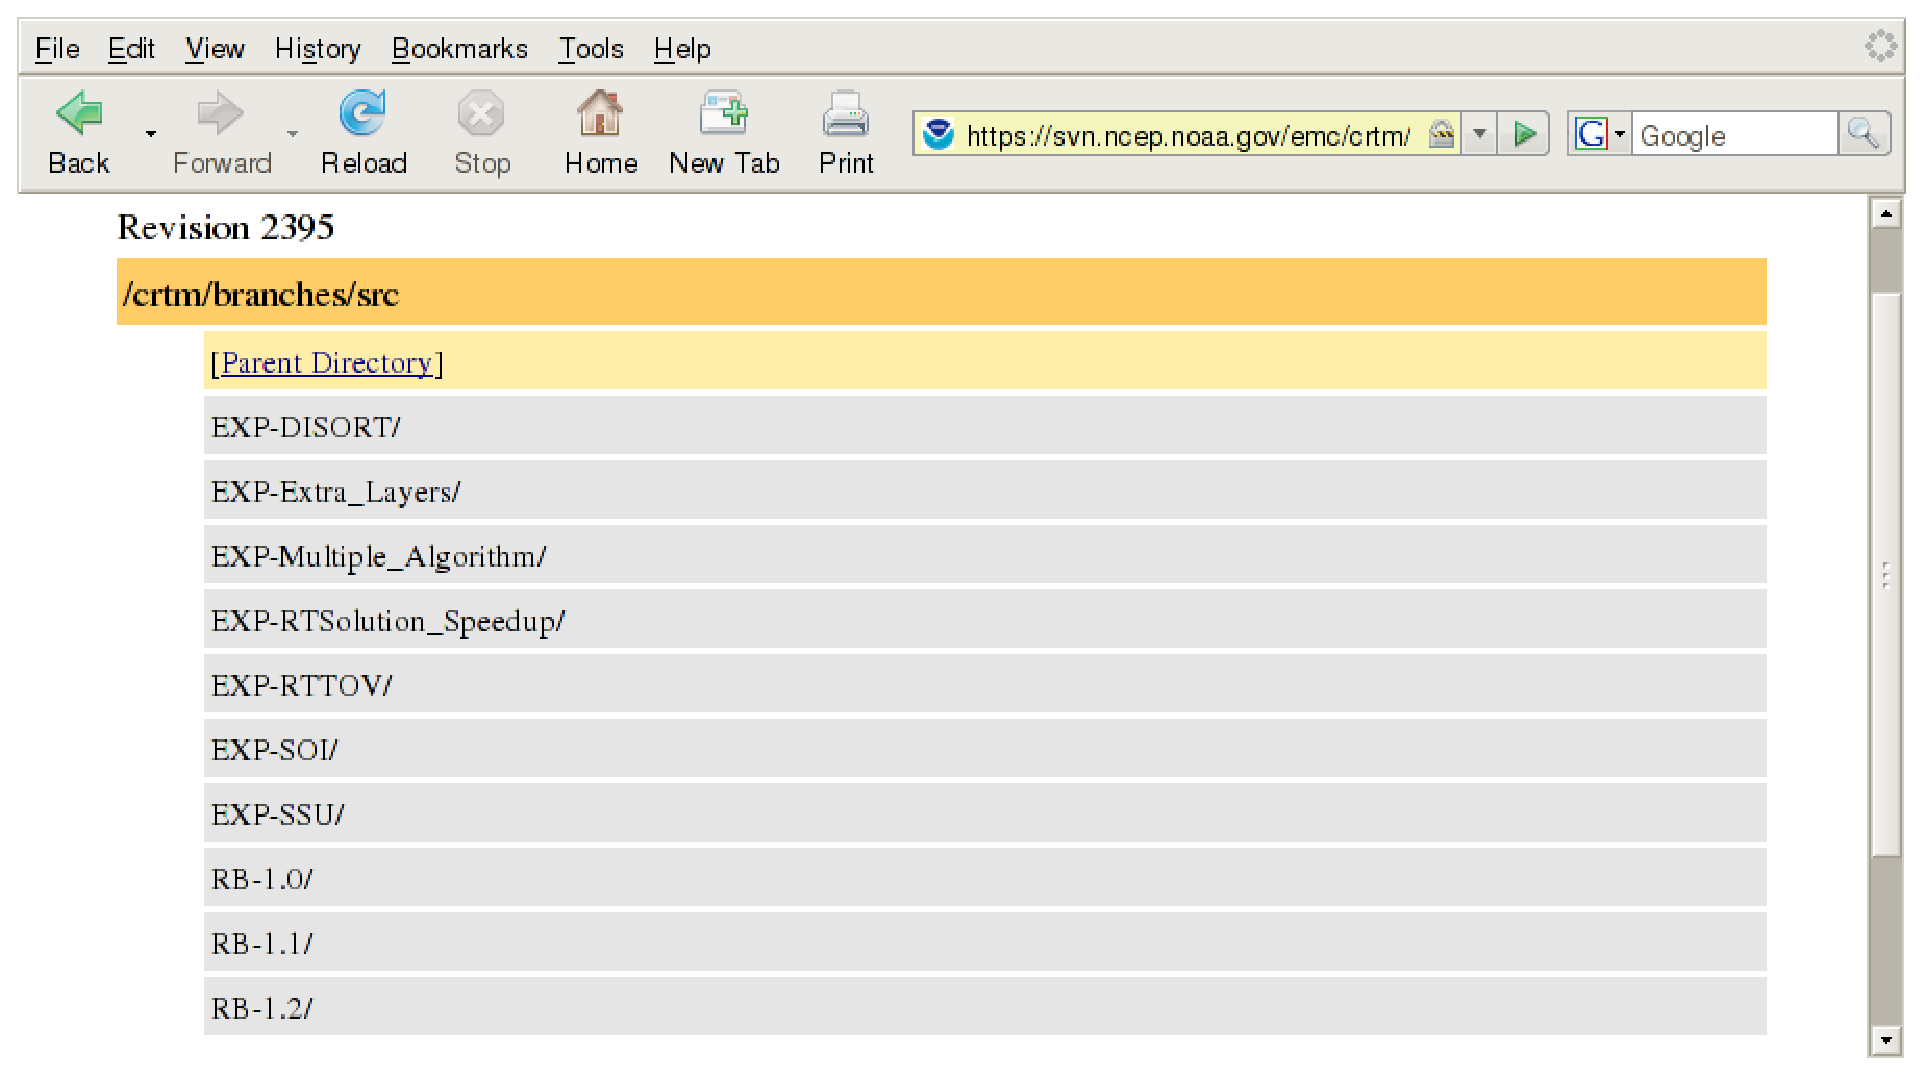
\includegraphics[scale=0.5]{graphics/branches_src_repository.eps}
  \caption{Snapshot of the \f{branches/src} subdirectory of the CRTM repository, showing the current branches.}
  \label{fig:branches_src_repository}
\end{figure}

\section{\f{tags} subdirectory}
%-----------------------------------
If a snapshot of development, or if development has been completed on a trunk or branch revision, a copy is made and placed in the \f{tags} subdirectory. There are three tag naming conventions in current use:
\begin{enumerate}
  \item For official software releases, \f{REL-}\textit{rel}; where \textit{rel} is the software relase number,
  \item For pre-release snapshots, \f{REL-}\textit{rel}\f{\_}\textit{stage}\f{.rev}\textit{RN}\f{.}\textit{YYYY-MM-DD}; where \textit{stage} is the release stage, typically \f{alpha} or \f{beta}; \textit{RN} is the repository revision number from which the tag was created; and \textit{YYYY-MM-DD} is the date on which the tag was created,
  \item For experimental branch snapshots, \f{EXP-}\textit{desc}\f{.rev}\textit{RN}\f{.}\textit{YYYY-MM-DD}; where \textit{desc} is a short description of the experimental branch.
\end{enumerate}
Some examples of the current tags in the CRTM \f{tags/src} subdirectory are shown in figure \ref{fig:tags_src_repository}. Note that there is no development in a tag directory - it is strictly a snapshot of a trunk or branch revision.

\begin{figure}[htb]
  \centering
  \includegraphics[scale=0.5]{graphics/tags_src_repository.eps}
  \caption{Snapshot of the \f{tags/src} subdirectory of the CRTM repository, showing the current tags.}
  \label{fig:tags_src_repository}
\end{figure}


\chapter{Build Conventions}
%==========================
This sections details the environment setup to enable the CRTM library, or any support software, to be compiled in a user's working copy. For the purposes of explanation, it will be assumed that a user's home directory is referred to by the environment variable \f{\$HOME}, and that the root directory of a user's working copy of the CRTM is \f{\$HOME/CRTM} and reflects the same directory structure as the repository.

\section{Macro Definitions}
%--------------------------
All of the makefiles in the CRTM repository use environment variables as required to locate the particular category subdirectories described in table \ref{tab:trunk_category_description}. The environment variable names, along with example definitions for a working copy are shown in table

\begin{table}[htb]
  \centering
  \begin{tabular}{p{4.5cm} p{9.5cm}}
    \hline
    \sffamily\textbf{Environment Variable Name} & \sffamily\textbf{Example Definition} \\
    \hline\hline
    \f{CRTM\_SOURCE\_ROOT}    & \f{\$HOME/CRTM/trunk/src}, \f{\$HOME/CRTM/branches/src/RB-1.2}\\
    \f{CRTM\_FIXFILE\_ROOT}   & \f{\$HOME/CRTM/trunk/fix} \\
    \f{CRTM\_TEST\_ROOT}      & \f{\$HOME/CRTM/trunk/test} \\
    \f{CRTM\_SCRIPTS\_ROOT}   & \f{\$HOME/CRTM/trunk/scripts} \\
    \f{CRTM\_EXTERNALS\_ROOT} & \f{\$HOME/CRTM/trunk/externals} \\
    \f{CRTM\_DOC\_ROOT}       & \f{\$HOME/CRTM/trunk/doc} \\
    \hline
  \end{tabular}
  \caption{Environment variables used by CRTM makefiles.}
  \label{tab:macro_description}
\end{table}

Ideally, the environment variables of table \ref{tab:macro_description} should be defined in a user's environment definition file to ensure they will be defined in any shell invocation.


Note the multiple examples for the \f{CRTM\_SOURCE\_ROOT} macro....


\section{Master Make Include Files}
%----------------------------------
All of the makefiles in the CRTM repository ....



\section{Install of script files}
%--------------------------------


\end{document}

